\chapter{State of the art}

    This chapter aims at providing a literature overview on the topics that are related to the main problem that this thesis aims to solve, which is the lack of communication between applications and the infrastructure where they reside.
    As such, the first section focuses on discussing means and structures through which nodes are organized in networks today, from which three were selected for their current popularity and their high potential for applicational traffic optimization : peer-to-peer (P2P) networks, content distribution networks (CDNs) and server-client networks that leverage server mirroring.
    For each of these, a conceptual analysis is made - more specifically, the context behind them, relevant concepts, architecture, and possible use cases.
    Additionally, there's an examination on how applications that utilize these networks affect, positively or negatively, the physical infrastructure where they operate, and if potential exists for mutually-beneficial layer cooperation.
    The following section displays existing proposals for increased layer cooperation, alongside a discussion of the practical consequences of adopting such proposals.
    The final chapter overviews the Application-Layer Traffic Optimization (ALTO) working group's proposal, which is a subset of the proposals of the previous section that contains more in-depth information, as it is the main inspiration of this thesis.

\section{Peer-to-Peer (P2P) Networks}

\subsection{Concepts and Applications}

    Due to the many hybrid implementations that have surfaced, the definition of a P2P network has become harder to pinpoint.
    Nevertheless, a P2P network is grounded on some definitions, among them that it consists on many singular computing elements, the "peers", which have among themselves similar privileges and functions (this contrasts with the client-server architecture, where two different roles exist - the one that is to be served and the one that is to serve - with functionality and control being thus centralized).
    P2P networks decentralize computational resources as a means to achieve certain tasks, and such resourcefulness of the entire system as a whole gives it an interesting list of properties, among them:

\begin{itemize}
    \item \textbf{Dynamic scaling}: As all member nodes can share their computing resources with the network, the system as a whole increases its capacity with increased users. Since the peers also act as clients to the network, scaling the service becomes less of a challenge as each new client will also act as a server. This also removes the necessity to manage how many service resources are needed - the amount of existing resources is linked to the number of existing clients, and thus there's no need to purchase and manage central resources, as the network dynamically allocates them by nature.
    \item \textbf{Resilience to failure}: Whereas centralized solutions are vulnerable to node and link failure, a P2P network can more easily work around such threats - as all peers can encompass the same server functionality, network services and resources are not dependant on a limited set on nodes, but instead redundantly deployed throughout.
    \item \textbf{Power decentralization}: As a direct consequence of computational and resource sharing, no single peer has direct control of the network, and the information is not centralized. As such, this considerably deters any attempts to overpower the network, e.g., via means of censorship or biased node favouring.
\end{itemize}

    These, however, are not without their nuance - since many P2P hybrids exist, these properties can change and others can appear.
    For example, if we consider BitTorrent, which has Tracker servers to redirect users to a correct peer with the requested resource, whilst the network itself can still be resilient to failure, the content-retrieval service that the P2P network provides has a single point of failure and of control - the trackers themselves.
    Furthermore, the P2P network design, by its nature, also has some issues to consider:

\begin{itemize}
    \item \textbf{Security:} The equal functionality property that P2P networks have give much power to peers to affect others. Without proper care, malicious peers are a security risk.
    \item \textbf{Management:} Since resources and services are not centralized, tasks such as event logging and resource backups become very difficult, and perhaps impossible if the peers do not abide to any orchestration protocol.
\end{itemize}

    P2P applications have had, in the past decades, a mainstream image that is plagued with legality and security issues.
    Nonetheless, when these are overcome the P2P networking strategy possesses many interesting properties - some of them displayed above - that make it fitting for varied use cases - e.g. file sharing, media streaming, social networking and problem solving via distributed and cooperative algorithms.
    More recently, P2P applications have been considered a fitting solution for low-cost content delivery systems in high demand scenarios, in applications such as PPStream and PPLive in China, which offer live video streaming through P2P with great success \cite{cisco}.

\subsection{Architecture}

    As stated previously, the term "Peer-to-peer" has become very broad and now serves as an umbrella for many different sub-types of systems.
    This chapter focuses on overviewing the architecture of many of these sub-types.
    All P2P networks are characterized by consisting of peers that know one another as to form a so-called overlay network on top of its supporting network.
    How peers are organized in these P2P networks and how they operate is what distinguishes the many sub-types.
    Table \ref{table:p2p-structures} groups known P2P applications in regards to their centralization and structure, as did \cite{p2p-survey-1} and \cite{p2p-survey-2}, with the latter further distinguishing the protocols in regards to other metrics, e.g., security, reliability, and performance.
    One would expect that all P2P applications would have no centralization at all, since the P2P design sees function and routing spread throughout the network.
    Alas, some modifications have been made in some of these sub-types, which shift how much decentralization they have.
    Similarly, different levels of structure are employed that shift the network's efficiency with how much structure is set in regards to its operation.
    As would be expected, these sub-types of P2P networks thus possess different strengths and weaknesses, and as such could be applied to different use cases.

\begin{table}[]
\caption{Types of P2P systems (Adapted from \cite{p2p-survey-1})}
\label{table:p2p-structures}
\begin{adjustbox}{max width =1.1\textwidth,center}
\begin{tabular}{lllllll}
                                                 &                                        &                                                                                 &                                                                                                                 &                                                                                                                          &  &  \\ \cline{3-5}
                                                 & \multicolumn{1}{l|}{}                  & \multicolumn{3}{c|}{Centralization}                                                                                                                                                                                                                                                                                          &  &  \\ \cline{3-5}
                                                 & \multicolumn{1}{l|}{}                  & \multicolumn{1}{l|}{Hybrid}                                                     & \multicolumn{1}{l|}{Partial}                                                                                    & \multicolumn{1}{l|}{None}                                                                                                &  &  \\ \cline{1-5}
\multicolumn{1}{|c|}{\multirow{9}{*}{Structure}} & \multicolumn{1}{l|}{None}              & \multicolumn{1}{l|}{\begin{tabular}[c]{@{}l@{}}Bittorrent, Napster,\\ Publius\end{tabular}} & \multicolumn{1}{l|}{\begin{tabular}[c]{@{}l@{}}Kazaa,\\ Morpheus,\\ Gnutella (extension proposals),\\ Edutella\end{tabular}} & \multicolumn{1}{l|}{\begin{tabular}[c]{@{}l@{}}Gnutella,\\ FreeHaven\end{tabular}}                            &  &  \\ \cline{2-5}
\multicolumn{1}{|c|}{}                           & \multicolumn{1}{l|}{In Infrastructure} & \multicolumn{1}{l|}{}                                                           & \multicolumn{1}{l|}{}                                                                                           & \multicolumn{1}{l|}{\begin{tabular}[c]{@{}l@{}}Chord,\\ CAN,\\ Tapestry,\\ Pastry\end{tabular}}                          &  &  \\ \cline{2-5}
\multicolumn{1}{|c|}{}                           & \multicolumn{1}{l|}{In System}         & \multicolumn{1}{l|}{}                                                           & \multicolumn{1}{l|}{}                                                                                           & \multicolumn{1}{l|}{\begin{tabular}[c]{@{}l@{}}Bittorrent (DHT/Trackerless), \\OceanStore,\\ Mnemosyne,\\ Scan, PAST,\\ Kademlia,\\ Tarzan\end{tabular}} &  &  \\ \cline{1-5}
                                                 &                                        &                                                                                 &                                                                                                                 &                                                                                                                          &  &
\end{tabular}
\end{adjustbox}
\end{table}


    Early versions of Gnutella come as a famous example of a decentralized and unstructured architecture, as peers act with equal functions and privileges, and no inherent structure exists on how these peers connect, store or retrieve content.
    The bootstrapping method consists on users reading from a set of known Gnutella peers, which is essentially a static list of addresses obtained from a trustworthy source, and attempting to connect to each one of them until a preferred number of known neighbours is reached.
    The unstructured nature of this protocol makes it so there's no systematic way to efficiently retrieve content, as thus peers must flood the network with content queries until either a reply is met or the predefined TTL value is exceeded.

    The author defines partially centralized architecture as similar to those which are decentralized, but with the added caveat that some peers are chosen to service a portion of the network.
    This is done to take use from the fact that not all network peers are alike in terms of memory, computational power, or other relevant resources.
    As such, more capable peers are elected as "supernodes" and are delegated with more responsibilities, noting that these self-configure in situations where such supernodes fail or willingly leave the network, and thus there is no single point of failure as there would be on a true centralized architecture.

    A hybrid architecture approach in a P2P network  employs some elements from the client-server architecture.
    With Napster as an example, whilst peers still operate as servers or clients, they must contact an intermediary - and central - server when querying for content, which will in turn redirect them to one or many peers that contain it.
    A similar concept applies for BitTorrent, where such intermediary servers are called trackers.
    Obviously, the choice to add a centralized aspect to the architecture hinders many of the advantages from a purely unstructured solution - namely its scalability, resilience to failure, and decentralization of control - as a trade-off to facilitate the control and maintenance of the network, as well as the peers' ability to bootstrap to it and locate content.

    A P2P architecture is structured if it systematically employs some non-random criteria on how the network operates, e.g., how peers organize themselves, where content is stored and how it it retrieved - for example, FreeNet uses the content's hash as a key that is used to query for it, and which is used by the peers in each subsequent hop to know where to forward the request, instead of flooding the network in attempts to blindly find it.
    Many of the structured P2P architectures rely on distributed hash tables (DHTs), which are structured ways to map a key to some content in the network, in such a way that the full key-space is partitioned over the peers.
    Two examples of structured P2P architectures that use DHTs can be seen in Figure \ref{fig:dht-usage} - to the left, the Chord algorithm uses a circular DHT where each peer knows the location of some peers that are their predecessors, and some that are their successors.
    When a peer needs to query for some content, it uses its key to firstly search for it locally and, if not, forwards the query to following peers, and the process recursively continues.
    To the right, the content addressable network (CAN) has the key-space mapped to a virtual two dimensional space, and its area is partitioned to peers considering their geographical location.
    A straight arrow from querying node to the node that has the content represents the routing path that the querying message must travel: A-B-E.

    Employing a systematic way to self-organize and share content is the means to guarantee that a P2P network can be fully decentralized whilst maintaining a desirable level of performance.
    However, the reliance on structure means that it must be maintained, e.g. managing neighbour pointers on Chord or managing area allocations on CAN, and that can be costly or even impossible with high rates of peer churn, i.e. with a sufficiently large rate of peers entering and leaving the network.

\begin{figure}%
\centering
\subfloat[Route of content query messages that originate at node 0 with destination at node 15, in the Chord system.]{{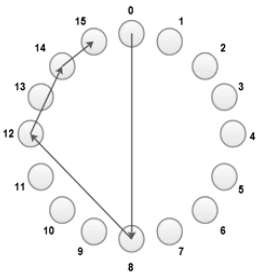
\includegraphics[width=5cm]{img/chord.png} }}%
\qquad
\subfloat[Route of content query messages that originate at node A with destination at node E.]{{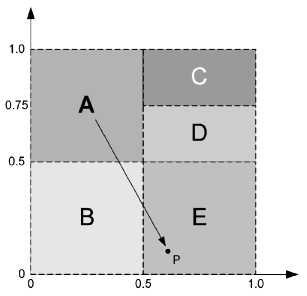
\includegraphics[width=5cm]{img/can.png} }}%
\caption{Examples of structured P2P systems that utilize DHTs}
\label{fig:dht-usage}
\end{figure}

\todo{make own version of these images}

\subsection{Effects to the Network Infrastructure}

\todo{liao2014}
\todo{falar de artigo de tussle}

    Historically, ISPs have deemed P2P traffic as unideal or even undesirable.
    Besides the aforementioned illegality precedent that is tied to P2P applications, the overall properties of P2P networks make them unappealing to support - due to the distributed nature of these types of networks, the overall traffic is less predictable, with the higher upload traffic volume in edge networks requiring infrastructural investments, and the network-agnostic operation mode of P2P applications leads to inefficient and uncooperative network resource usage.

    P2P networks who neither have structure nor a central point of control have to utilize content retrieval methods which are bound to be less efficient than their counterparts.
    However, architectures which fit in these categories mostly do so with a clear purpose - Gnutella's decentralized nature makes it very hard for individual nodes or external entities to regulate what can happen in the network (such as enforce legal actions), and its lack of structure simplifies the architecture and reduces the overall effort to bootstrap to the overlay, making it a good fit for applications with a high peer churn rate.
    Similarly, FreeHaven's architectural decisions fit a very specific use case, as it "emphasizes distributed, reliable, and anonymous storage over efficient retrieval" \cite{freehaven}.
    The lack of systematic means to efficiently locate content by these P2P architectures means that more ad-hoc methods have to be used, which are less efficient and thus incur in bigger workloads for ISPs - the usage of query flooding by Gnutella and message broadcasting by FreeHaven are examples of this.

    The usage of structure by P2P networks can, as stated before, result in more efficient content and peer location algorithms.
    However, maintaining such structure also requires a chunk of ISP resources, as peers need to periodically update others, as well as react to peers entering and leaving the overlay.
    The usage of key-value mappings with DHTs is also ISP unfriendly as the hash function's purpose is to evenly distribute resources over the network - whilst such property is certainly advantageous in certain use cases, doing so removes any  applicational context that exists in the content - for example, grouping resources which belong to the same web page can't be done, as they will be individually hashed and spread out.

    Regardless of the P2P system operating under structural means or using a central point of control, no classic P2P system operates in full cooperation with ISPs.
    The network-agnostic manner under which they operate results in overlay networks which are layered on top of the underlay where they run, as exemplified in Figure \ref{fig:overlay-underlay} - as P2P applications are network-agnostic, two neighboring peers could exist in completely different contexts on the common network layer - for example, both being physical neighbours or distancing many network providers are possible scenarios.

\begin{figure}[!h]
\centering
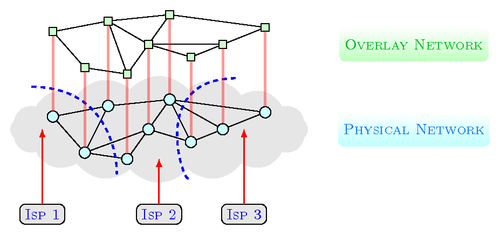
\includegraphics[scale=3.0]{img/p2p-topology.png}
\caption{Example demonstration of an overlay network and corresponding physical layer.}
\label{fig:overlay-underlay}
\end{figure}

\todo{Make my own version of this}

    In the theme of P2P applications not considering the underlying infrastructure emerges the issue of locality unawareness, i.e., the lack of knowledge on how much a given resources or nodes in the overlay actually distance themselves in the underlay.
    This issue is particularly damaging in P2P applications whenever neighbours are selected, and whenever a resource exists redundantly in the network and a decision must be made in regards to what file chunks to retrieve from what peers.
    If it indeed is the case that P2P applications are not locality aware, it can easily be seen how this can be an issue: for P2P applications, choosing peers which are not local to the querying peer may result in more time to retrieve the requested contents; for ISPs, bad network resources management can incur in higher operational costs, and may degrade overall network performance in many cases, e.g., overusing inter-AS links which usually are network bottlenecks (a conventional wisdom demonstrated in \cite{akella}).
    If the P2P application were to attempt to choose the peers that would most effectively serve the querying peer, it could depend on privileged information that the ISP has on the network's properties and current status (such as link load, scheduled tasks, or scheduled maintenance).
    Attempting to optimize peer selection without a co-operational channel with ISPs would be sub-optimal as not enough information is known, and could perhaps even be more damaging with the wrong techniques - consider a peer selection algorithm that chooses the peers with lowest RTT of a probing ping message, whilst having no indication on available end-to-end bandwidth.
    Likewise, attributing neighborship via geographical proximity - much like the CAN architecture - whilst initially seems like a good step in location awareness, may also not be optimal - ISPs may not always prefer geographical proximity in connections, as peers could be very geographically close but residing in different ASs and thus separated by costly links.
    Other peer-selection techniques focus on randomly selecting nodes, which is simple and resilient to peer churn \cite{qin2009}, but as a consequence is sub-optimal on network resource usage as no network consideration exists.
    It is fair to say that no P2P application can act with full ISP consideration without directly cooperating with it, and simple heuristics should be, whenever possible, traded for methods where full cooperation with the underlay is done - that is, if the needs of both layers are being considered.

    Indeed, it is the case that current P2P solutions are ISP-unfriendly, resulting in large amounts of upstream and downstream traffic.
    To name a few examples, BitTorrent seems to employ peer selection algorithms which do not consider the underlay network, which can result in degraded download performance and increased load on ISPs \cite{qin2009}.
    \cite{karagiannis} found that since this protocol is locality unaware, 70-90\% of existing local content was found to be downloaded from external peers and suggests that locality-aware content distribution algorithms could significantly reduce the total amount of traffic generated; also, Gnutella generates traffic which is not ideal, as it may have to cross ISP network boundaries multiple times \cite{estimating-gnutella} due to the same fundamental issue stated before - an application layer that operates in disregard to the network underlay it runs on.

    As \cite{dan-Commag10} describes, the ongoing friction between the overlay and underlay layers has made it to the point where ISPs have chosen to throttle the bandwidth of P2P traffic, or even outright blocking it.
    In return, P2P applications have tried to mask their presence to bypass such restrictions via tunnelling or using non-standard and random port numbers.
    This is an unsustainable system that is bound to hurt both ISP profit and application functionality, and a strategy of cooperation between the overlay and underlay layers is crucial to guarantee that the requirements of both parties are met.


\section{Content Distribution Networks (CDNs)}

\subsection{Concepts and applications}

    A content distribution network (CDN), as the name implies, is a network specifically designed with its  main focus on distributing content to a set of end users.
    Its design allows for the alleviation of performance bottlenecks on the Internet generated by client requests, and has been recently been considered a powerful tool as a response to the existing high demand for media-like content consumption that takes a huge share of the global Internet traffic of today.
    The current focus of CDNs is thus to provide content, e.g., web pages, documents, photos, videos, or even media-related streams, with high availability and performance.
    The strategy used by CDNs to guarantee a satisfying quality of experience (QoE) on a global scale is the deployment of content close to the end-user - a CDN contains many nodes which are geographically spread throughout the globe and close to the users they wish to serve, and whenever such users request for content, they are routed to the node which is closest to them (\cite{cookbook}).
    Data replication to servers which are strategically placed closest to end-users, coupled with good means to properly redirect such users to the most attractive edge server, is what allows content to be available more often and more quickly, which are undoubtedly attractive features in the world of e-commerce, where user QoE can dictate much of the profit - for example, Akamai, one of the leaders in CDN-related services, ran a research concluding, among other things (\cite{akamai}):

\begin{itemize}
    \item A 100 millisecond slower webpage loading speed can result with a 7\% drop in sales
    \item A 2 seconds slower webpage loading speed can almost double the number of visitors who end up abandoning their carts
    \item 53\% of users who use smartphones to visit web stores won’t make the sale if the webpage takes more than 3 seconds to fully load
    \item 28\% of users won’t return to the same web store if they think it takes too long to load
    \item A 250 millisecond faster loading time proved to keep users from visiting a competitor web store
\end{itemize}{}

    It should then come to no surprise that streaming services such as Netflix and Youtube, who now reach a global scale and whose utility is highly dependant on their high availability and low transmission delay, routinely use CDN solutions \cite{cookbook}.
    Indeed, companies that wish to provide some service in the web and who wish to have global presence routinely partner with companies whose focus is providing content delivery services, with popular examples being Akamai, CloudFlare, or Amazon Cloudfront.
    Coupled with the promise of highly available and quick content retrieval, these companies also couple other attractive services, such as firewalls and DDoS protection.
    The Internet's currently most targeted use for media consumption has made it so CDNs and their providers have an important role in dictating a very considerable percentage of flow of traffic in ISP-owned infrastructures, and as such their study and improvement is quite important, as are the efforts to increase harmonious behaviours between content delivery applications and service providers of the networks where the CDNs are deployed, with the goal in mind being network resource efficiency to guarantee that ISPs can remain operational and applications can provide a satisfiable user experience.

\subsection{Architecture}

    Whilst implementations may vary, Figure \ref{fig:cdn-architecture} shows a high level representation of most CDN solutions.
    Delivery nodes possess the data which is to be requested by end-users, and are usually deployed as close to the demand points as possible, as discussed before.
    Such content is provided to the delivery nodes by the storage nodes which in turn are retrieved by the content's source.
    Integral to the operation are the control nodes, which are responsible for managing, routing and monitoring the CDN, being the role responsible for dictating how it operates.
    Content can be provided to delivery nodes before any request for it occurs in areas where its request can be predicted to exist, via push operations, or requested at the same time as it is also done by the client, via a pull operations, and subsequently cached.
    Additionally, a continuous request for data can be made by such edge nodes whenever a data stream is requested \cite{cdn-guide}.

\begin{figure}[!h]
\centering
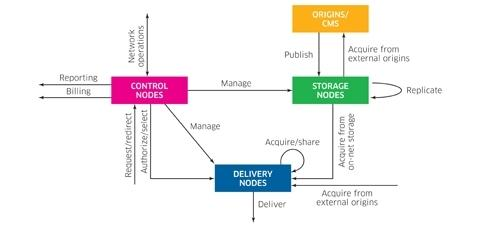
\includegraphics[scale=8.0]{img/cdn-architecture.jpg}
\caption{high level architecture of a CDN (adapted from \cite{global-dots})}
\label{fig:cdn-architecture}
\end{figure}

    Request routing is the mechanism through which clients and located and mapped to a given CDN edge server.
    The prevalent approchaces are, according to \cite{wichtlhuber2017}, the following:

\begin{itemize}
    \item \textbf{DNS request routing}: The user must first resolve a domain name to retrieve a content. The CDN's DNS processes such request and, utilizing the user's IP address, historical measurement information and current server loads, responds with the edge server that seems most fitting to provide such content.
    \item \textbf{HTTP request routing}: Content is firstly requested to a nearby proxy server, which in turn answers with an HTTP redirect to be resolved by the client in order to find the content. The HTTP requests can occur in subsequent rounds and can also use DNS knowledge when the redirection domain must be resolved.
    \item \textbf{Anycast request routing}: The CDN provider announces an anycast prefix to the network. Whenever a router receives multiple announcements to the same prefix incoming from different locations, it chooses one considering some custom criteria, usually being AS hop count and Interior Gateway Protocol (IGP) weight.
\end{itemize}{}

\subsection{Effects to the Network Infrastructure}

    As previously discussed, CDNs came as a tool to strategically position content in such a way that it can more quickly and more reliably be retrieved by an end-user.
    The usage of CDNs are of great interest by ISPs as their mode of operation, if made properly, can be very appealing not only to them but also to end-users.
    The usage of a single content-providing server (or a limited set of them) which is far away from the content supply that can have large number of points that are scattered throughout the globe, is prone to overloading such server and path congestion if a big enough scale is achieved.
    The usage of data caches is a classic solution for network inefficiency problems which is also used by CDNs as a means to replicate content to strategic locations to better serve users, with the added benefit for ISPs that their network resources are efficiently used, reducing the total amount of used bandwidth needed for a service to operate, as data travels a shortened total amount of network hops from data source to points of data demand.
    It can thus be stated that the relationship between CDNs and ISPs are a win-win situation because efficient network usage has consequentially better service quality.
    However, attributing edge servers to end-users entirely on geographical data was previously discussed as being a non-optimal way of assessing node selection at the application layer.
    Whilst it may be intuitive that the best edge server to serve an end-user would be the one most geographically close to it, that is not always necessarily the case, much like was discussed in similar strategies used in P2P systems.
    Again, much like in the scenario of peer selection in P2P systems, the usage of network measurements made by the CDN itself to better pick the appropriate end-server, while it could potentially be beneficial, it could certainly be improved if it used additional, hard to retrieve data that only ISPs or other privileged entities could possess, and which are at a position to guide applications in the infrastructure with whom they have detailed knowledge.
    Acting with regards to the underlying network structure would be beneficial to better optimize server selection in a way that is mutually beneficial to the overlay and underlay.
    Whilst the problem of server allocation becomes easier with a smaller number of deployed end-nodes - e.g., choosing an edge server may be trivial if there's one per continent - as the number of these increases with user demand, it becomes more important to optimize server selection in a way that is dynamic and finely tuned to the network where it operates.

\todo{pros and cons to different request routing techniques}

\todo{find examples where CDNs misbehave regarding ISPs or at the very least struggle to optimize network traffic}

\section{Server mirroring}

\subsection{Concepts and applications}

    Server mirroring is the act of continuously replicating a server into another, essentially creating an exact copy of it that is now accessible as if it were the original.
    Whilst CDNs aim at replicating chunks of contents wherever it may be necessary, the act of server mirroring performs an integral copy of a server which is self sufficient at serving a given client, as long as it periodically checks up with the primary server for synchronization \todo{cite}.
    It is a standard business strategy that uses redundancy as a means to increase reliability, availability and performance.
    The existence of many servers that perform the same task means that these can be strategically chosen to serve a client in a given situation, e.g., by selecting the one that has small end-to-end message delay and little current server load.
    Figure \ref{fig:mint-mirrors} shows an application of this, where multiple server mirrors exist to deliver software packages to the Linux Mint distribution. The user has the choice to manually select one of these mirrors, and ideally chooses the one that is most fitting to them.

\begin{figure}[!h]
\centering
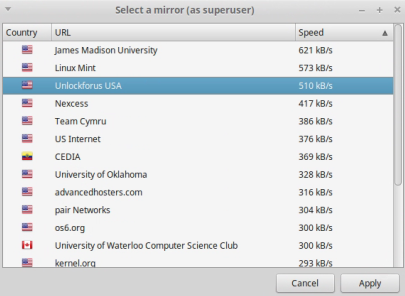
\includegraphics[scale=1.0]{mint-mirror.png}
\caption{Linux Mint prompt to select a software repository mirror}
\label{fig:mint-mirrors}
\end{figure}

\subsection{Effects to network infrastructure}

    Much like the content replication utilized in CDNs, an integral replication of a main server proves itself as an advantageous tool capable of delivering services more closely to users, and as such allows the reduction of total amount of bandwidth used to serve all clients.
    Much like all previous use cases discussed before, optimizing application traffic is crucial to guarantee good network resource usage, and in case of server mirroring it comes down to good strategical deployment and dynamic, intelligent algorithms to properly attribute mirrors to requesting end-users.
    Giving end-users the choice to manually select the serving mirror seems problematic, as application-generated traffic is not optimized.
    In fact, considering the Linux Mint software package distribution discussed above, despite currently existing seventy mirrors deployed throughout the globe to fit this role, a large number of these remains mostly unused whilst the main and default server is constantly prone to overworking \cite{mint-article}.
    It can be stated that end-users both don't care enough to optimize traffic nor do they have enough information to properly do so even if they did.
    Deployment of server mirrors is a great tool that brings with it the issue of optimizing server selection, and much like all examples given so far, traffic generated by applications can be firstly optimized by the applications themselves if they consider static and dynamic information of the network they operate on.

\section{Traffic optimization by applications and layer-cooperative approaches}

    This section serves to display the proposed solutions and existing implementations that have been made in the attempt to optimize application traffic utilizing network information.
    Given the increasing scale of the Internet as a near ubiquitous system, and increasing tension between service providers and applications, it comes as no surprise that the area of layer cooperation has been through exhaustive work.
    Many solutions have been devised for specific use cases, with varying degrees of power to each one of the layers.

    Many different mechanisms have been developed with the goal of decreasing tensions between ISPs and P2P applications, which is a subset of the general layer cooperation problem.
    Figure \ref{fig:p2p-isp-interactions} represents a grouping proposed by \cite{dan-Commag10} where such mechanisms are ordered in agreement with how much involvement the P2P systems and ISPs have. These classes are as follows:

\begin{itemize}
    \item \textbf{Class 1}:
        There is not much interference in the overlay by ISPs nor are P2P systems cooperative.
        Instead, ISPs apply traffic engineering methods to selectively favour types of traffic.
        This is usually done to guarantee certain QoS levels to some classes of traffic, which are then to be treated favourably at the forwarding and routing levels.
        Examples of such techniques are DiffServ, Multi-Topology Routing (MTR) and MultiProtocol Label Switching (MPLS).
        These classes of methods do not fix the underlying problem, but are instead used to control preexisting traffic.
        As such, the peers' routing decisions are not affected and and P2P traffic still remains non localized.
    \item \textbf{Class 2}:
        There is ISP intervention in the overlay in such a way that peers continue normal operation without realizing that such interventions occur.
        This can be reached via the use of proxies that can effect the control plane with the redirection of content requests to local peers, or at the data plane with content caches which act as normal peers and are strategically placed in the network.
        These methods are advantageous because they do not require any changes to P2P protocols, because the ISP has an active role in molding to the overlay, intercept traffic, and either help or guide it in a way that favours them.
        Indeed, these techniques can be proven to work , as concluded in \cite{dan-Commag10}, and put into practice, for example, in \cite{programmable-trackers} and \cite{configurable-trackers} via the specification of a BitTorrent tracker that is programmable to allow for P2P qualitative differentiation and ISP-cooperative traffic engineering that could help reduce inter-domain traffic significantly.
        However, this class of mechanisms are not without their challenges - firstly, it involves much effort by ISPs, as it requires structural upgrades and constant adaptiveness to new and changing P2P protocols.
        Perhaps worse, even considering proper budget and maintenance, such methods can prove themselves to be not possible at all - for legal reasons, as data caches could possibly contain illegal content; and for technical reasons, since the packet inspection required by ISPs to detect and steer P2P traffic may be blocked due to the peer's attempts to mask its traffic as non-P2P related.
    \item \textbf{Class 3}:
        Relative to previous classes, the active role is switched, and it is the P2P system itself that acts in regards to the underlay it operates on, but without ISP involvement, which would require change from classic P2P protocols.
        Peers probe the neighboring network elements as a way to get more familiar to connection properties, and act on these probings during operation, e.g., when choosing neighbours to construct the overlay network on when choosing where to retrieve a given resource.
        Whilst these methods can be advantageous for both applications and ISPs, it can't be assumed that to always be the case.
        As peers have no ISP input, they cannot have a full scope on the network and ISP needs, and as such these application optimizations can end up being more hurtful than helpful.
        For example, this paper mentions a simple scenario where a peer uses RTT measurements to choose between two candidate peers, but the one that is geographically closest to it belongs to another AS, and his selection would incur in more costs.
        The paper describes this class as a "win-not-lose" situation, meaning that while the P2P system can, in the right circumstances, improve its performance via measurement, the ability to act beneficially to the underlay without any feedback from ISPs cannot be guaranteed.
        such a example of improved performance could be seen at \cite{qin2009}, which improved BitTorrent's download performance and even managed to reduce ISPs' backbone and cross-ISP traffic.
        The technique consisted in having peers send traceroute measurements to the tracker, which in turn grouped them into local, intra-ISP and inter-ISP groups, with the assumption that inter-ISP links generally have much more latency than the rest.
        As peers would later query the tracker for content, the returned peer list would be biased in such a way that promotes traffic locality.
    \item \textbf{Class 4}:
        Full and active cooperation exists between the ISPs and P2P systems.
        The role of the ISPs is to provide information, and P2P systems let that information dictate its decisions.
        It is the methodology that most comes close to a mutually advantageous scenario for both parties, given that they both keep the entire group's needs in mind.
        For example, \cite{locality-aware-p2p} proposes an oracle that receives as input from querying peers a list of candidate peers, and ranks them in order of proximity to the querying node; such method was tested in simulation and proven to decrease negotiation traffic and improve scalability of P2P networks.
        Another example of this is \cite{kim2011}, which devised a CDN-P2P hybrid where peers utilize RTT measurements to group themselves by separate orders of geographical proximity with the same intent of the previous example, which is to localize traffic whenever possible.
        This technique also proved itself to be advantageous, as the solution was more efficient in terms of total service disruption time when compared to a previous iteration of the hybrid architecture which used random peer selection to look up available target peers.
        The functional intent is that the oracle possesses privileged network information and acts on it to provide guidance to querying applications, and thus has the liberty to impose policies and optimizations, e.g., pair peers which are the least number of network hops apart via a Dijkstra algorithm.
        Another more complex approach that could be used by the oracle proposed by \cite{han2009}, which contains algorithms to dictate peer selection, task assignment and rate allocation.
        The method requires the full network topology as input - including link capacities and peer service costs - to minimize file downloading time and cost.
        The oracle would also be free to enforce ISP biases as it desires by modifying such algorithms as to, for example, minimize usage of costly links (such as inter-AS ones).
        The ALTO working group - whose work this thesis attempts to materialize into a working library and further extend its features - was formed to standardize the oracle-user scenario so it could be properly used in many situations at the scale of the Internet as a whole.

\end{itemize}

\begin{figure}[!h]
\centering
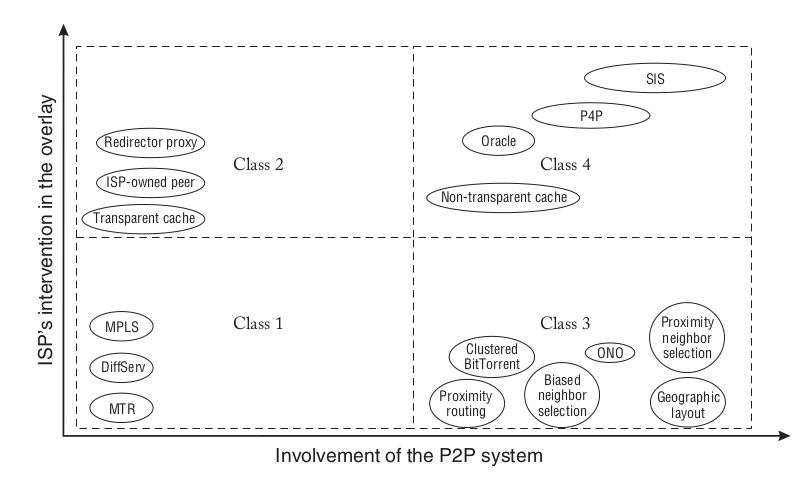
\includegraphics[scale=0.65]{img/approaches-isp-p2p.png}
\caption{Existing approaches to decrease tension between P2P applications and ISPs (\cite{dan-Commag10})}
\label{fig:p2p-isp-interactions}
\end{figure}

    Given the current share that CDNs have on global Internet traffic of today, coupled with the demand for a good QoE by end-users, it should come to no surprise that this applicational domain has also been through efforts to optimize its traffic.
    One such way to do so is to optimize client query redirection, i.e., better choose which edge server should be attributed to an end-user when a name resolution is requested for some content.
    \cite{gromov2014} considers a CDN built to deliver video data where some given set of content exists redundantly in many edge-servers, and argues for an algorithm where the choice is made to optimize client download time, which in turn has to consider the network parameters at time of request, as well as current server load.
    In another angle, IETF devised a problem statement in regards to Content Distribution Network Interconnection (CDNI) \cite{cdni-problem-statement}, which outlines the efforts needed to specify a set of interfaces that allow for the interconnections of many CDNs, with the added benefits that a multi-CDN system will have better availability, coverage, and capabilities than the single CDNs by themselves.
    The four devised interfaces (CDNI Control interface, CDNI Request Routing interface, CDNI Metadata interface, and CDNI Logging interface) are all control plane interfaces to be operated at the application layer, and the group states that no new application protocol needs to be devised, and instead existing ones could be leveraged, e.g., HTTP, Atom publishing protocol, XMPP, and in particular to the CDNI Request Routing interface, the ALTO protocol who's the focus of this work.
    Still in the topic of optimizing CDN's edge server selection, \cite{wichtlhuber2017} suggests a way of optimizing anycast request routing, which differs from the DNS-oriented request routing techniques, which, while very light in terms of network engineering and infrastructural overhead when compared to existing alternatives whilst maintaining a close to optimum network path, it sacrifices flexibility to do so, as it is agnostic to the network's status and not much network engineering can thus be done.
    As such, the work proposes anycast request routing utilizing software defined networking (SDN), where load balancing is made at the ISP network with help of CDN-provided aditional information.
    This example of layer cooperation can allow for many optimization opportunities that leverage an existing and low-maintenance mean of request routing with the flexibility achieved with SDN solutions.

    Attempting to optimize web server selection, \cite{kenichi} argues that DNS-oriented solutions, which select the nearest server but also employing load balancing, may not be the best at optimizing server-client QoS levels.
    Instead, it is proposed that selection is based on QoS measurements, from which three types are distinguished: a static method, such as choice based on least number of hops to server (which is unlikely to change); a dynamic method, consisting on dynamic instantaneous probing of the network to monitor, for example, round-trip time (RTT) delay to the servers; and statistical methods, which decide based on a larger set of measurements made in various points in time.
    Utilizing the latter method, RTT measurements and web-related request benchmarking is made, such as time to establish TCP connection, elapsed time from GET HTTP method to first packet received, time to retrieve data fully, etc, every five minutes and spanning several weeks.
    The work concluded that statistical methods used to select between multiple equal web servers had high correlation with download time from the selected server, but optimizations should be evaluated in regards to computer workload and the amount of probing traffic.
    Tackling a similar challenge, \cite{swain} proposes a method of server mirror selection which is better optimized than the more popular approach of giving the user the selecting choice.
    Thus, the proposed solution's architecture consists of two types of agents: a client agent, which monitors the mirror server it was deployed in and stores static information, e.g., geographical location of server and maximum capacity, and dynamic information, e.g., current load and bandwidth.
    This information is then sent to the other role of the architecture, the server agent, which compiles it and acts as an oracle that is queried by users whenever mirror selection is needed, replying with a ranking of candidate servers based on bayesian networks.

    Congruent to the task of optimizing network traffic with layer cooperation, \cite{adaptable-overlay} proposes a reconfigurable and adaptable overlay multicast system, further optimizing the multicast strategy - used for group communication as a means to reduce redundant traffic - and leveraging collaborative efforts between it and the ISPs to construct multicast distribution trees whilst integrating traffic engineering mechanisms for the task of network usage optimization.

\section{Application-Layer Traffic Optimization (ALTO) working group}

\subsection{Context and Motivation}

\todo{alto for determining service edge (2x)}
\todo{alto for locating caches}

    Following research indications that improved peer selection algorithms based on ISP-provided information could help reduce ISP costs and increase P2P application performance, the Internet Engineering Task Force (IETF) devised working groups to explore IETF standardization in the area of layer-cooperation \cite{seedorf2009}.
    Among them is the Application-Layer Traffic Optimization (ALTO) working group, whose domain is traffic localization.

    The ALTO working group designed an HTTP-based application protocol whose function is to allow hosts to query privileged servers on network information.
    The envisioned scenario of the service provided by the ALTO architecture, as can be seen on Figure \ref{fig:alto-design}, considers both the physical and application levels.
    The ALTO service is provided by some oracle, which needs to be himself informed on network information that can take many forms - topological structure, routing costs considering many metrics, static provider policies, etc - and, most importantly, such data is to be fed by an ISP, or another entity that contains truthful and relevant network information that the oracle could deem useful in aiding its clients.
    Consider that "Peer 2" has to choose, among "Peer 1" and "Peer 3", which peer to retrieve a resource from (the information of what peers contain the resource in question could've been retrieved from a tracker or via a flooding query).
    Instead of resorting to classical strategies, such as random choice or probing measurements, "Peer 2" is to use the ALTO service, querying the oracle on information pertaining to the candidate peers, and in regards to metrics that better fit the needs of the application (because different applications could have different QoS metric priorities in mind, such as a media stream with low delay needs or a file sharing application with focus on bandwidth).
    Ideally, it would make sense that the querying peer would end up choosing "Peer 3", as they reside on the same network.
    As could be deduced from this and similar scenarios, an architecture containing one or more servers that are knowledgeable on the network they reside on could be an important tool to make P2P applications locality-aware.

\begin{figure}[!h]
\centering
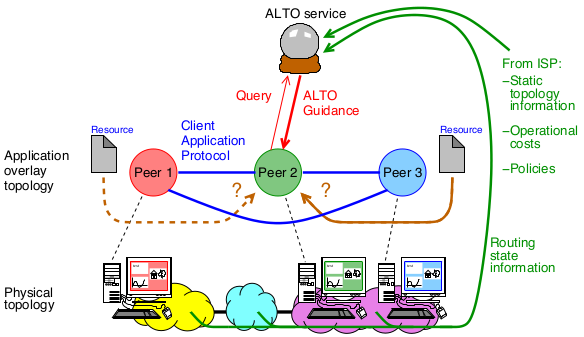
\includegraphics[scale=0.75]{alto-design.png}
\caption{ALTO scenario \cite{seedorf2009}}
\label{fig:alto-design}
\end{figure}

    Despite the origins of the ALTO protocol lying in P2P applications, it is now being considered in other fields, such as data-center networks and content distribution networks (CDNs) \cite{alto-about}.
    With interest in the latter example, ALTO protocol extensions are being developed as a means to create functionality that could be useful for services employing CDNs, most specifically the implementation of the CDNI Request Routing Footprint \& Capabilities Advertisement interface \cite{alto-cdni}, which is a subset of the CDNI standard \cite{cdni-problem-statement} that aims to allow upstream CDNs to query known downstream CDNs if they are able and willing to accept the content request.
    In particular, one of the main functionalities of the CDNI request routing interface is the ability for upstream CDNs to retrieve static or dynamic information on download CDNs (resources, footprint, load), which they provide themselves, and that allow upstream CDNs to better choose the appropriate edge server that could serve a given end-user.
    ALTO serves as a good protocol to implement such functionality because it fits its use-case: some node (in the upstream CDN, where the content query originates) wishes to improve its routing (in regards to resolving content requests) by using information, which is hard to deduce by itself, to properly choose the most efficient node (the downstream CDNs where the content resides).
    At a more abstract level, this is similar to the use case fulfilled to P2P applications to help them better select peer connections.

    A mode of operation where applications no longer operate in disregard to the network infrastructure they run on, but instead in deep consideration of it, could help significantly alleviate the issues emerging from the tension between the underlay and overlay levels, and is of mutual interest - improving application performance and reducing infrastructural costs.
    Enabling a communication channel can thus allow for many different co-operational use cases besides the aforementioned ones - for example, redirecting users to nearby data caches or warning them of server maintenance ahead of time.
    The existence of an all-encompassing oracle could also prove beneficial for applications which utilize periodic network probing to guide their choices, as such information could be made by a select few nodes in the network and applicable to all nodes which are close-by to such node in ways that the ISP seems advantageous (such as belonging to the same AS or geographically near), thus minimizing the amount of probing traffic used and giving it to an entity that could better reason with it to help the querying user.

    Finally, standardizing an architecture and related protocols that could help a large subset of problems could also be of great value as it would facilitate the integration of solutions into other ones which already follow the specified standard, thus leveraging the ALTO protocol to their needs, not requiring further cycles of development.
    Also, in a more abstract level, the attempt to standardize is helpful as it joins forces from many different domains which share common patterns (many exemplified previously), and as such could result in a better and more proven product that could be used at the scale of the Internet itself.

\subsection{Architecture}

\todo{adicionar jsons exemplos em apendice?}

    The general ALTO architecture can be seen on Figure \ref{fig:alto-architecture}.
    Central to the operation is the ALTO server, which stores network information and provides it to querying clients.
    Such network information is provided by trustworthy entities, with some enumerated in the same figure.
    Two protocols can be seen as part of the general architecture: the provisioning protocol, not contemplated by the ALTO working group, should specify how information is provided to the ALTO Server; the ALTO protocol, main focus of this working group, specifies server-client interactions mainly in the form of data querying and delivering.
    The ALTO client is the main consumer of the ALTO service as a whole, and it queries the ALTO server on network information whenever it deems such data as necessary to what it's doing at a given moment.
    An ALTO client could be seen as any entity which is able to interface with the ALTO protocol as the role of a client, and as such is not tied to a specific implementation - in the example of P2P file sharing, a peer can act as an ALTO client (like the example scenario in Figure \ref{fig:alto-design}), but instead a tracker could enhance its role in assisting peer communication by having an embedded ALTO client which would then act on behalf of querying peers as to provide them with an optimal response.

\begin{figure}[!t]
\centering
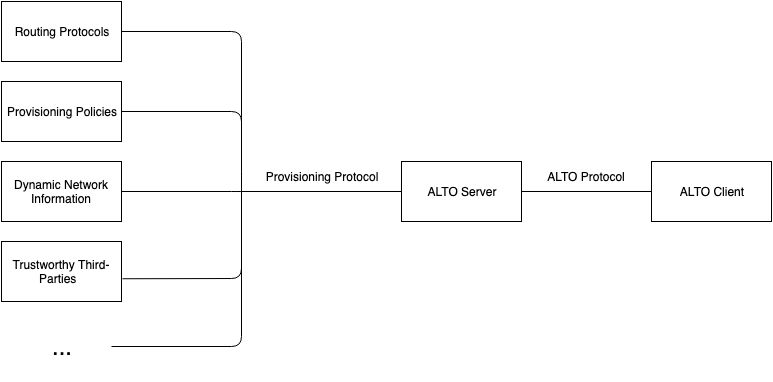
\includegraphics[scale=0.60]{alto-architecture.jpeg}
\caption{ALTO architecture (adapted from \cite{alto-protocol}) }
\label{fig:alto-architecture}
\end{figure}

\newpage

    The ALTO services contemplated by the corresponding working group can by visualized in Figure \ref{fig:alto-services}.

\begin{figure}[!h]
\centering
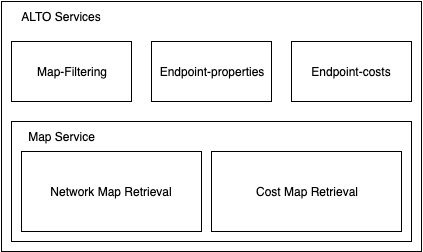
\includegraphics[scale=0.55]{alto-services.jpeg}
\caption{ALTO services (adapted from \cite{alto-protocol}) }
\label{fig:alto-services}
\end{figure}

    The ALTO server stores and provides special mappings in the form of network and cost maps.
    A network map provides network location grouping identifiers and the corresponding aggregated endpoints.
    It utilizes Provider-Defined Identifiers (PIDs) as a key, and the mapping itself is left to the responsibility of the providers - it is thus a way of indicating that many endpoints should be handled similarly.
    A provider can then aggregate endpoints by geographical proximity, one or many subnets, one or many Autonomous Systems (ASs), etc., and attribute properties to the aggregate, instead of the endpoint.
    The other resource type provided is a cost map, which can be defined as a matrix M, where $M_{ij}$ - with i and j being the source and destination PIDs, respectively - is the associated path cost between the two indexes.
    The cost has two components: its metric and mode.
    The ALTO base protocol only defines a single, generic, cost metric called "routingcost".
    However, the current draft \cite{alto-metrics} is, as time of writing, currently specifying more concrete metrics, with many associated with Quality of Service (QoS) evaluation, e.g. one way and round trip delay, packet loss and throughput.
    The other cost property, cost mode, can either specify that the metric is to be interpreted as a numerical value or as an ordinal ranking among all other costs in that cost map - this is useful in cases where too much network information is not deemed reasonable to share, and a simple order of preference that doesn't expose too much infrastructural detail can suffice.
    The decision to separate network and cost map information into two types of resources comes from the reasoning that network mappings are unlikely to change, whereas cost mappings could be periodically updated.
    As such, it alleviates client applications from the need to retrieve redundant information, and the ability to only retrieve a subset of it - this ability is further expanded in the map filtering service, which allows an ALTO client to further specify which regions of the requesting maps it wishes to retrieve (much like a "SELECT" statement from the Structured Query Language (SQL)), and only these are transmitted to it.

    Finally, the last two services focus on mappings that regard to specific endpoints, instead of abstract mappings that utilize PIDs.
    An endpoint is identified by one of the following: IP address, MAC address, or overlay ID.
    The endpoint property service maps to an endpoint a set of properties, e.g., geographical location or connectivity type, and the endpoint cost map has the same meaning of a cost map, but mapping to particular endpoints and not abstract collections.


    As could be seen, the ALTO project specifies an architecture for trading of network-related information, with well defined roles and a request-response protocol to fulfill interactions between them.
    It also attempts to standardize such interactions in the form of data structures with well defined attributes which are then to be manipulated for each use case.
    This could then serve as a useful service for any application that wishes to retrieve network information that could improve its decision making at the application level.
    It is important to note that there are restrictions to what kinds of information are contemplated by the ALTO protocol - for example, transport-level congestion is beyond its scope, and thus should not replace conventional mechanisms.
    The type of data which is valid to consider, according to \cite{alto-protocol}, should not be easily obtainable by the clients themselves (such as end-to-end delay), and should be variable on a longer timescale than the instantaneous kinds that are seen on congestion control, as the resulting intelligence gathering traffic generated would be counterproductive to the task of traffic optimization.
    Potentially valuable information that is in the ALTO scope would then have to be harder to obtain without aid of this service, and not highly mutable through time - for example, routing costs, geographical locations, network proximity, operator's policies, scheduled down-times, etc.

    This project is, at time of writing, still on-working, with many drafts being published and updated.
    These are, however, relating to service extension and deployment, as the main architecture, protocol design, implementation guidelines and security analysis are fully published into their respective RFC documents.

\subsection{Viability}

\subsubsection{Security}

    Given the nature of this architecture - the trading of sensitive network structure information that can alter application behavior - it is quite apparent that its implementation is not without challenges from a security perspective.
    As such, \cite{alto-protocol}, besides over-viewing the protocol, also does a threat analysis of the ALTO architecture.
    Utilizing the "STRIDE" threat model, the main threats to the ALTO architecture are as follows:

\begin{itemize}
    \item Spoofing of a legitimate ALTO server that would mislead clients with wrong information - this could give the malicious party the ability to change traffic to its will.
        Spoofing of the clients themselves can also occur, and could allow a malicious party to retrieve sensitive network data they aren't authorized to.
    \item Tampering of data to mislead either ALTO servers or clients.
        If some unauthorized and malicious party can retrieve data that is in transit and tamper with it, clients would act on information that they assume if trustworthy but in fact has been modified.
        As such, clients could be redirected to wrong addresses, or receive incomplete or incorrect data that results in bad decision making.
        On the other hand, data tampering that occurs between data providers and the ALTO server would give it, a seemingly trustworthy party, untrustworthy data.
        This would result in the same issues pointed previously.
    \item Repudiation of being the source of some network information, whether it be by a third party or the ALTO server itself, would make it difficult to neutralize and attribute culpability to incorrect or malicious sources.
    \item Information disclosure in the form of ALTO resources made available to entities that were not in the authorization circle.
            These resources could give malicious parties insight on network topology status as well as the ability to derive clients' network usage patterns by observing what kinds of resources they attempted to retrieve in a given moment.
    \item Denial of service (DoS) of the ALTO server itself via the creation of more requests than it can handle, as well as via the manipulation of ALTO resources themselves - if a cost map is manipulated to highly favor a specific subset of servers, these could be favourably picked by clients in a disproportionate matter, and highly affect these servers' availability.
    \item Elevation of privileges that lead to obtaining or modifying more information than initially permitted.
\end{itemize}

    Many of these threats are standard and could be solved with state of the art solutions which are well proven and tested, as indeed states \cite{alto-protocol}.
    However, threats of information disclosure - whilst they can be negated with in-transit encryption, what is done with this information the moment it reaches the client is hard to control.
    Situations may arise when a privileged client shares, intentionally or not, sensitive network information it retrieved from an ALTO server to an unprivileged client.
    Furthermore, many differently privileged clients could share information among themselves which they initially retrieved legitimately, to get a complete view of the network structure. Thus, individual clients could internally cooperate to bypass the access control measures applied by the server.
    As such, it is firstly important for the ISP or third parties that provide such information to carefully plan out the network state it wishes to share, and how granular of a state is actually provided.
    Possible solutions to minimize these threats are as follows:

\begin{itemize}
    \item Reduce the variety of the provided data, with the consequence of less precise ALTO guidance
    \item Provide information that refers to abstraction instead of concrete data.
        One example is the usage of network groupings by PIDs instead of information mapping to concrete endpoints.
        Another example is the usage of ordinal cost types that indicate relative preference instead of concrete cost values.
        This strategy suffers from the same downsides as the previous one
    \item Work only with a small set of trustworthy ALTO clients that are to act on behalf of a larger subset of less trustworthy clients.
        For example, via the deployment of certified trackers that choose on behalf on P2P clients by giving them customized responses.
        This is still, however, worthy of a threat analysis as many relative information could be derived from the clients via carefully crafted requests.
    \item Utilize terms of agreements that are to be enforced on every querying client.
        This would work as a dissuasion method but could be infeasible and impractical if other threats are not neutralized (such as spoofing).
        Furthermore, such enforcement could be seen as unappealing by some users as it could violate user privacy.
\end{itemize}

\subsubsection{Privacy}%

    Privacy concerns are also very prevalent in the ALTO system.
    When an ALTO client queries a server for one or more resources in the attempt to optimize the application traffic it will generate in the near future, certain parameters can be passed to the server that can make the response be more personalized and contain more granular information.
    For example, a P2P media-streaming application seeking ALTO guidance to help choose between candidate peering neighbors may wish to include in its query the list of candidate peers it is considering connecting to, the fact that the querying application prioritizes real-time communication, and the network position of the querying client itself.
    Indeed, these and more patterns will help increase the effectiveness of the ALTO server's guidance in helping the client application achieve its goal, but such happens at the expense of potentially allowing an ALTO server to infer on user pattern statistics.
    Even assuming that the previously discussed information disclosure threats are nonexistent in the ALTO system, privacy concerns can arrive from client applications because the resource queries they need to produce can contain information about what the client either will or wants to do.
    This is recognized by the ALTO working group as a possible concern \cite{alto-protocol} \cite{alto-problem-statement}.
    In response, they state that the clients should firstly be cognizant about the potential tracking risk that is associated with the usage of the system and, as an attempt to make tracking harder, they could disable HTTP cookies and/or opt for more vague query information, e.g. by randomizing some bits on endpoint addresses or simply using more broad addresses, but being aware that the helpfulness of query results may change with increased parameter obfuscation.
    Provider-Defined Identifiers (PIDs) were created as a means for ISPs to abstract network components as a collection of single network endpoints with similar properties, helping them not to disseminate network information that is too sensitive, and in turn also allows clients to make queries based on these identifiers and maintain a higher level of privacy.
    Other solutions could also be considered depending on the needs of the clients and the direction of the project as a whole.
    For example, the servers themselves could leverage a secure communication channel and maintain a clear agreement on what can and cannot be made with the collected information, or even if it is collected at all.
    Alternatively, clients that wish not to impose much trust on server could make bulk queries (or use proxies to do so for them) and privately filter out the relevant information.

\subsubsection{Incentivization}
\todo{collaboration problem}
\todo{ALTO servers could be egotistical in how they steer peers}
\todo{the voluntary nature of the system makes it risky}

\subsubsection{Network Neutrality}

%    \cite{dan-Commag10} raises important challenges related to the cooperation between ISPs and P2P systems, with some being applicable to the ALTO system as the ALTO server acts as an oracle in Class 4 of the interaction groupings made by the author.
%    In particular, three of the concerns have yet to be stated here and are very relevant on the topic of the ALTO system's viability, and as such will now be brought up in the following topics.

    Network neutrality has been a popular point of discussion as society grows around the Internet, sparking debates around the world on what the best course of action should be - for example, regulations were introduced by the FCC in the United States \cite{fcc} to police network neutrality, and the European Union has a framework for net neutrality laid down by article 3 \cite{article-3}.
    However, potential violators of the spirit of a network neutrality exist, such as British Plusnet's usage of deep packet inspection (DPI) to implement limits and differential charges for different traffic \cite{arstechnica}, or Portuguese MEO's smartphone contracts which include zero rating programs for a given set of services \cite{meo-packages}, as displayed on Figure \ref{fig:meo-dataplan}.
    Network neutrality advocates are concerned with guaranteeing that ISPs keep Internet communications free and do not discriminate based on the traffic's specifics, such as platforms, applications, or source or and destination.
    As stated by \cite{qos-framework}: "According to most network neutrality proponents, network neutrality rules are intended to preserve the Internet's ability to serve as an open, general-purpose infrastructure that provides value to society over time in various economic and non-economic ways. In particular, network neutrality rules aim to foster innovation in applications, protect users' ability to choose how they want to use the network, without interference from network providers, and preserve the Internet's ability to improve democratic discourse, facilitate political organization and action and to provide a decentralized environment for social, cultural and political interaction in which anyone can participate.".
    On the other hand, opponents of net neutrality, among them ISPs, broadband and telecom companies, and hardware manufactures, argue against net neutrality.
    They claim that it would would reduce incentive to invest, as investments would be harder to insure without the ability to charge higher rates for better infrastructure capabilities.
    Zero rating programs, such as Wikipedia Zero, which provides Wikipedia with no charge to a select group of low income regions \todo{cite} , would also not be possible.
    Additionally, with net neutrality, the ISPs' ability to route traffic could itself be at jeopardy - as \cite{jerzy} states in their solution to compromise net neutrality with QoS demands via service differentiation, the Internet is growing at an astonishing rate, as are the QoS demands of applications, and operating the infrastructure on a purely best-effort basis will not be sufficient without a constant provisioning of such infrastructure to keep up with demand, and this may not be viable nor even possible.
    Thus, discriminating traffic services may be needed to guarantee that, say, real-time medical information gets priority over real-time media streaming, which in turn gets priority over e-mail or file sharing.
    Considering that the ALTO system behaves in an oracle pattern of cooperation where a single entity - the ISP - is able to heavily influence the traffic patterns of the applications it aids, on the promise of a symbiotic network underlay-overlay relationship, such system could violate the principles of net neutrality.
    In particular, this could happen if the oracle intends to block or discriminate a given type of traffic, such as deliberately giving better guidance to certain types of applications.
    A possible consequence of such a system guiding the Internet could be that given applications can consistently have better QoS measurements not on the basis of the application's implementation, but on the ISPs personal biases.
    These biases could also be applied to the end-users where guidance requests originate, thus resulting in two clients in equally capable network areas getting different QoS measurements simply because the ISPs decided as such.
    Oracle systems such as ALTO do not seem to be analogous to other traffic engineering strategies, such as the usage of MPLS, DiffServ, nor to other means of ISP intervention on overlays, such as the deployment of data caches and redirector proxies.
    This is because the oracle system, in contrast to the previously mentioned strategies, is one of mutual voluntariness and cooperativeness between ISPs and applications.
    However, it could be argued that if the ALTO system offered guidance to applications in such a way that consistently resulted in better application performance, such applications would be pressured to use such guidance as a means to remain competitively viable, and the ISPs would then have a platform to influence a considerable amount of traffic to their will, being in a position to, depending on how they treat guidance requests, break network neutrality.
    This concern can be alleviated if application guidance operated on classes of traffic, e.g. real-time communication or file sharing, thus operating on traffic aggregates to insure QoS levels needed to given application types, but never discriminating beyond such given classes.
    This is, in fact, what happens with ALTO cost maps, whose metrics include, for example, round-trip delay, loss-rate, hop-count, or throughput \cite{alto-cost-metrics}, thus allowing different types of applications to request whichever cost types seem most suitable for their use case, with insurance that guidance is agnostic to where the guidance request comes from, or what application requests it.

\subsubsection{Multi-Domain orchestration}
    The Internet as we know it today spans the entire globe and is rather complex in nature.
    According to \cite{dan-Commag10}, the classic vision of the Internet consisting of a network of transit and stub ASs no longer seems accurate, as it now is much more complex - for starters, the role of network owner and service provider are separating, and Internet access is provided by numerous competing ISPs.
    As a demonstration of such complexity, \ref{network-connectivity-globe} displays how the Internet is structured into many tiers of different service providers.
    It can thus be seen that the act of layer cooperation can get harder when the cooperation domain increases and potentially spans many different ISP regions which will inevitably act differently when queried for council - for example, in regards to what network information they're comfortable with sharing, internal policies, what they aim to get out of the cooperation, etc.
    These per-ISP biases can make it difficult to guarantee that traffic optimization spanning multiple administrative domains is actually useful and achieves the symbiotic nature in mind.
    For example, an ISP may not be comfortable categorising end-point costs of a given metric, thus making path calculations that pass through that ISP domain not viable.
    Even assuming that all ISPs are comfortable with sharing such information, ambiguity may arrive - considering a cost map with the generic "routingcost" metric considered in the main protocol, ISPs could internally calculate routing costs differently, and prioritizing different goals, e.g. reducing overall link usage versus reducing inter-AS traffic first and foremost.
    The base ALTO protocol specification states that each network region can provide its ALTO services, which in turn convey network information from the perspective , with a network region consisting of, for example, an AS, an ISP, or a given set of ISPs \cite{alto-protocol}, thus implying that if multiple ISPs share an ALTO server they also share the perspectives they wish to share.
    Furthermost, the ALTO working group's deployment considerations document states that an ALTO client can query a single server for one or many metrics, or he can additionally query multiple server instances on different network instances \cite{alto-deployment-considerations}. It is explicitly stated in the document that each server could give guidance for only a given network partition, and such guidance may wildly differ between them due to the fact that different algorithms and objectives may have been applied.
    The document also states that, in regards to guidance synchronization, three different strategies could be applied:

\begin{itemize}
    \item \textbf{Authoritative Servers}: A given set of servers can provide guidance for all kinds of destinations to all ALTO clients.
    \item \textbf{Cascaded Servers}: An ALTO server can possess an embedded ALTO client and query other ALTO servers if its own guidance ability is lacking some information, acting as a proxy for the guidance received by a third entity.
    \item \textbf{Inter-server Synchronization}: Different ALTO Servers communicate among themselves to expand the knowledge space.
\end{itemize}

    The last strategy is still being subject to development and standardization by the working group as part of a bigger attempt to link different network regions and technologies into a single, homogeneous abstraction of the Internet.
    Current efforts and relevant use case examples are summarized in \cite{ALTO-multi-domain-use-cases}.

\todo{Falar da nossa tentativa, se lá surgirmos}

